\renewcommand{\thesection}{\arabic{section}}\renewcommand{\theHsection}{chapter.\arabic{section}}\setcounter{section}{5}\section{刚体的运动}
\noindent\begin{minipage}{\textwidth}\ProblemHeading{例题}{6.1（改写）}
设 $I_1,I_2,I_3$ 为刚体相对于质心的三个主转动惯量。证明任意一个主转动惯量不大于另外两个主转动惯量之和。
\end{minipage}\par\vfill
\noindent\begin{minipage}{\textwidth}\ProblemHeading{例题}{6.2（改写）}
设刚体的质量分布关于通过质心的平面 $\Pi$ 镜面对称。
\SubQ{1}{证明可以选取两条惯性主轴位于 $\Pi$ 内，第三条垂直于 $\Pi$。}
\SubQ{2}{若刚体由全部位于 $\Pi$ 内的质点组成，设两条面内主轴的主转动惯量为 $I_1,I_2$，求垂直于 $\Pi$ 的主轴的转动惯量 $I_3$。}
\end{minipage}\par\vfill
\newpage
\noindent\begin{minipage}{\textwidth}\ProblemHeading{习题}{6.3}
把分子看作由彼此距离保持不变的质点组成的系统。对下列各情形，求分子相对于质心的三个主转动惯量。
\SubQ{1}{分子由位于一条直线上的原子组成。以原子质量 $m_a$ 和它们的两两距离 $l_{ab}$ 表示结果。}
\SubQ{2}{三个原子位于等腰三角形的三个顶点。底边长为 $a$，高为 $h$，两个底角处的原子质量均为 $m_1$，顶角处的原子质量为 $m_2$，见第一幅图。}
\SubQ{3}{四个原子位于正三棱锥的四个顶点。等边三角形底面边长为 $a$，高为 $h$，底面的三个原子质量均为 $m_1$，顶点原子的质量为 $m_2$，见第二幅图。}
\begin{center}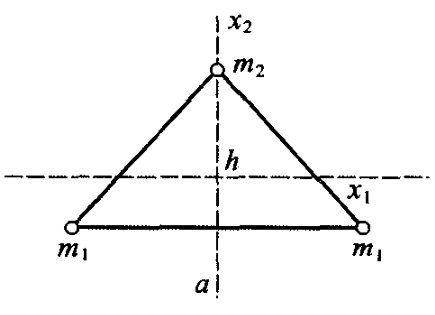
\includegraphics[width=0.25\linewidth]{figures/fig_6_3_1.png}\qquad 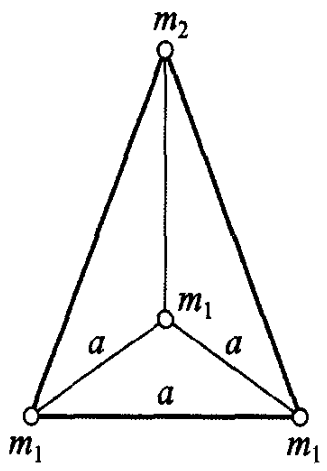
\includegraphics[width=0.18\linewidth]{figures/fig_6_3_2.png}\end{center}
\end{minipage}\par\vfill
\noindent\begin{minipage}{\textwidth}\ProblemHeading{习题}{6.4}
求下列质量均为 $\mu$ 的均匀连续体相对于质心的三个主转动惯量。
\SubQ{1}{长为 $l$ 的细直杆，横截面尺寸可忽略。}
\SubQ{2}{半径为 $R$ 的实心球。}
\SubQ{3}{底面半径为 $R$、高为 $h$ 的实心直圆柱。}
\end{minipage}\par\vfill
\newpage
\noindent\begin{minipage}{\textwidth}\ProblemHeading{习题}{6.5}
求下列质量均为 $\mu$ 的均匀连续体相对于质心的三个主转动惯量。
\SubQ{1}{棱长分别为 $a,b,c$ 的长方体。}
\SubQ{2}{底面半径为 $R$、高为 $h$ 的实心直圆锥。}
\SubQ{3}{半轴长分别为 $a,b,c$ 的实心三轴椭球。}
\end{minipage}\par\vfill
\noindent\begin{minipage}{\textwidth}\ProblemHeading{习题}{6.6}
一个质量为 $\mu$ 的刚体在重力加速度为 $g$ 的均匀重力场中绕固定水平轴摆动。质心到该轴的距离为 $l$，相对于质心的主转动惯量为 $I_1,I_2,I_3$，这三条惯性主轴与水平转轴的夹角分别为 $\alpha,\beta,\gamma$。求这个物理摆在稳定平衡位置附近的微小振动频率。
\end{minipage}\par\vfill
\newpage
\noindent\begin{minipage}{\textwidth}\ProblemHeading{习题}{6.7}
两根质量均为 $\mu$、长度均为 $l$ 的均质细杆 $OA$ 和 $AB$ 在 $A$ 点铰接。$OA$ 可绕固定点 $O$ 在图示平面内转动，$AB$ 的端点 $B$ 沿 $Ox$ 轴运动。设 $\varphi=\angle AOB$，求系统的动能。
\begin{center}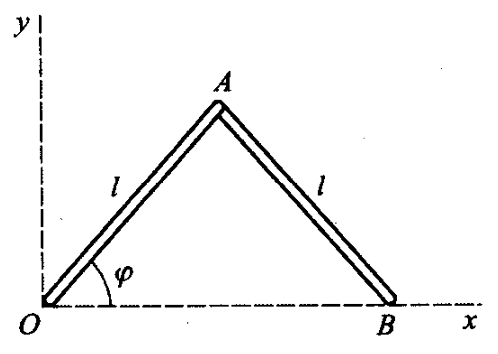
\includegraphics[width=0.31\linewidth]{figures/fig_6_7_1.png}\end{center}
\end{minipage}\par\vfill
\noindent\begin{minipage}{\textwidth}\ProblemHeading{习题}{6.8}
一个质量为 $\mu$、半径为 $R$ 的圆柱在固定水平面上作无滑动滚动。圆柱有一条穿过质心的惯性主轴与几何轴平行，两轴相距 $a$，绕该惯性主轴的转动惯量为 $I$。设在截面内从几何轴指向质心的线段与竖直向下方向的夹角为 $\varphi$（见图），求圆柱的动能。
\begin{center}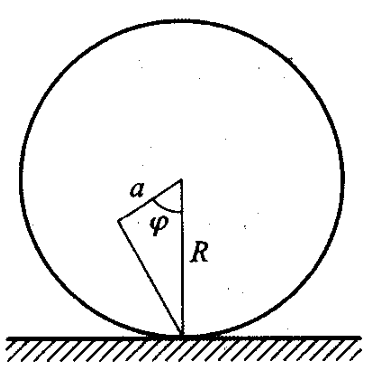
\includegraphics[width=0.28\linewidth]{figures/fig_6_8_1.png}\end{center}
\end{minipage}\par\vfill
\newpage
\noindent\begin{minipage}{\textwidth}\ProblemHeading{习题}{6.9}
一个质量为 $\mu$、半径为 $a$ 的均质圆柱，在固定的半径为 $R>a$ 的圆柱形曲面内侧作无滑动滚动，两圆柱轴线平行。横截面内从外圆柱中心到内圆柱中心的连线与竖直向下方向成角 $\varphi$（见图）。求滚动圆柱的动能。
\begin{center}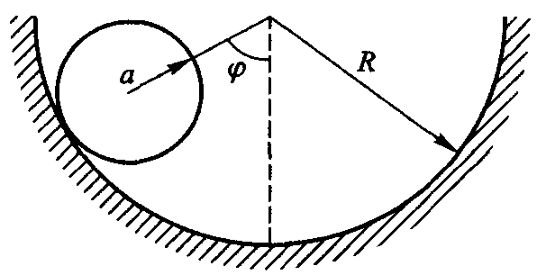
\includegraphics[width=0.33\linewidth]{figures/fig_6_9_1.png}\end{center}
\end{minipage}\par\vfill
\noindent\begin{minipage}{\textwidth}\ProblemHeading{习题}{6.10}
一个高为 $h$、顶角为 $2\alpha$、质量为 $\mu$ 的均质直圆锥，以侧面在固定平面上作无滑动滚动。设圆锥的接触母线 $OA$ 和平面内某一固定方向的夹角为 $\theta$（见图）。求圆锥的动能。
\begin{center}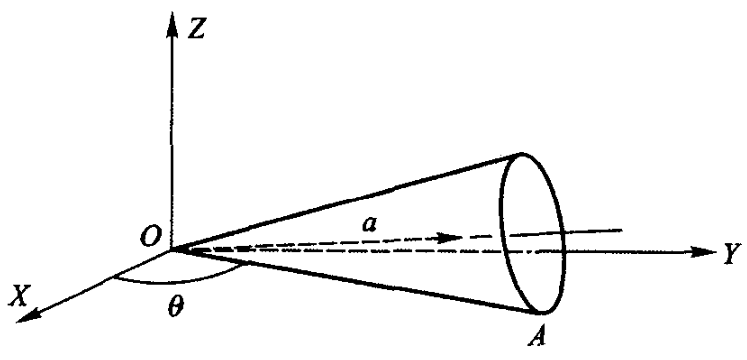
\includegraphics[width=0.37\linewidth]{figures/fig_6_10_1.png}\end{center}
\end{minipage}\par\vfill
\newpage
\noindent\begin{minipage}{\textwidth}\ProblemHeading{习题}{6.11（校订）}
一个质量为 $\mu$、高为 $h$、顶角为 $2\alpha$ 的均质直圆锥，以底面圆周在固定平面上作无滑动滚动。其圆锥轴始终平行于此平面，且顶点 $O$ 固定在离平面等于底圆半径的高度。设 $\theta$ 为圆锥轴的平面投影与平面内固定方向的夹角（见图）。求圆锥的动能。
\begin{center}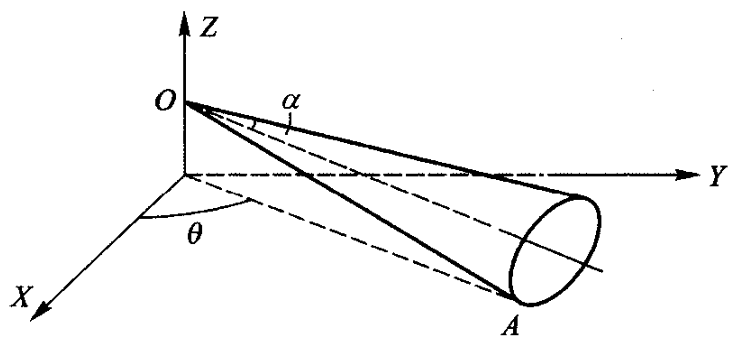
\includegraphics[width=0.37\linewidth]{figures/fig_6_11_1.png}\end{center}
\end{minipage}\par\vfill
\noindent\begin{minipage}{\textwidth}\ProblemHeading{习题}{6.12}
均匀二轴椭球绕一条自身的惯性主轴 $AB$ 旋转，$AB$ 又绕过椭球中心并与它垂直的直线 $CD$ 转动（见图）。取 $x_3$ 沿 $AB$，$I_1,I_2,I_3$ 为相对于质心的主转动惯量，$\varphi$ 为 $CD$ 与惯性主轴 $x_1$ 的夹角，$\theta$ 为绕 $CD$ 的转角。求椭球的动能。
\begin{center}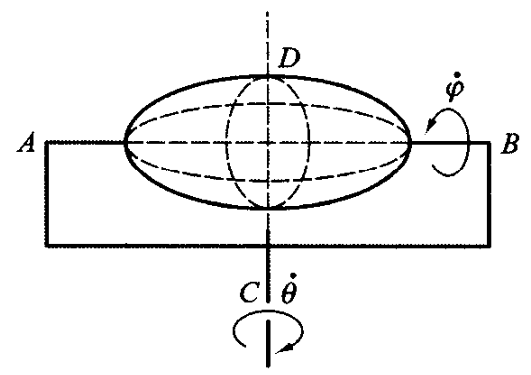
\includegraphics[width=0.31\linewidth]{figures/fig_6_12_1.png}\end{center}
\end{minipage}\par\vfill
\newpage
\noindent\begin{minipage}{\textwidth}\ProblemHeading{习题}{6.13}
均匀旋转椭球绕自身的对称轴 $AB$ 旋转，角速度为 $\dot\varphi$；$AB$ 同时绕过椭球中心的竖直轴 $CD$ 转动，角速度为 $\dot\theta$。$AB$ 与水平面的夹角恒为 $\alpha$（见图）。设相对于质心的轴向与横向主转动惯量分别为 $I_3$ 与 $I_1$，求椭球的动能。
\begin{center}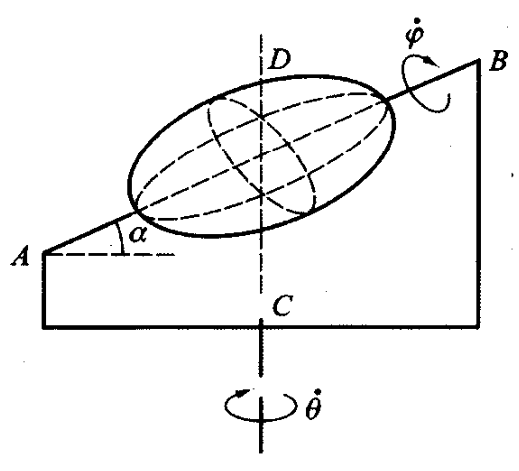
\includegraphics[width=0.31\linewidth]{figures/fig_6_13_1.png}\end{center}
\end{minipage}\par\vfill
\noindent\begin{minipage}{\textwidth}\ProblemHeading{例题}{6.14（改写）}
在质心参考系中考虑两种不受外力矩的刚体。用动量矩守恒说明各自的转动方式。
\SubQ{1}{相对于质心的三个主转动惯量相同的球形陀螺。}
\SubQ{2}{全部质点都位于同一条直线上的非静止转子。}
\end{minipage}\par\vfill
\newpage
\noindent\begin{minipage}{\textwidth}\ProblemHeading{例题}{6.15（改写）}
一个刚体由若干质点组成，位置矢量为 $\mathbf r_a$ 的质点在均匀力场中受到外力 $\mathbf f_a=e_a\mathbf E$，其中 $\mathbf E$ 是常矢量，$\sum_a e_a\ne0$。求一个作用点，使作用于此点的合力与原力系具有相同的力矩；分别说明在均匀电场和均匀重力场中的物理含义。
\end{minipage}\par\vfill
\noindent\begin{minipage}{\textwidth}\ProblemHeading{例题}{6.16（改写）}
相对于质心的主转动惯量为 $I_1=I_2$ 和 $I_3$ 的对称陀螺作自由转动，动量矩 $\mathbf M$ 不为零。取固定轴 $Z$ 沿 $\mathbf M$，动轴 $x_3$ 沿陀螺的对称轴。设 $\theta$ 为 $Z$ 与 $x_3$ 的夹角，$\varphi$ 为进动角，$\psi$ 为绕 $x_3$ 的欧拉角。
\SubQ{1}{用动量矩的各分量说明 $\theta$ 为常数。}
\SubQ{2}{当 $0<\theta<\pi$ 时，求 $\dot\varphi$ 及角速度在 $x_3$ 轴上的分量 $\Omega_3$。}
\end{minipage}\par\vfill
\newpage
\noindent\begin{minipage}{\textwidth}\ProblemHeading{习题}{6.17}
一个质量为 $\mu$ 的对称重陀螺以对称轴上的下端点 $O$ 为固定点，在重力加速度为 $g$ 的均匀重力场中运动。质心到 $O$ 的距离为 $l$，关于质心的轴向和横向主转动惯量分别为 $I_3$ 和 $I_1$。取固定轴 $Z$ 竖直向上，欧拉角如图。求解陀螺的运动，可以用积分给出结果。
\begin{center}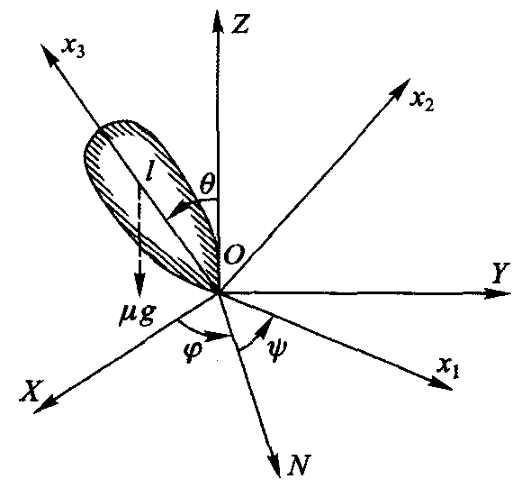
\includegraphics[width=0.33\linewidth]{figures/fig_6_17_1.png}\end{center}
\end{minipage}\par\vfill
\noindent\begin{minipage}{\textwidth}\ProblemHeading{习题}{6.18}
一个对称重陀螺的下端点 $O$ 固定，质量为 $\mu$，质心在对称轴上且距 $O$ 为 $l$，关于质心的轴向和横向主转动惯量分别为 $I_3$ 和 $I_1$。当它的对称轴竖直向上，陀螺以角速度 $\Omega_3$ 绕此轴转动时，求这种直立转动对小倾斜扰动保持稳定的条件。设重力加速度为 $g$。
\end{minipage}\par\vfill
\newpage
\noindent\begin{minipage}{\textwidth}\ProblemHeading{习题}{6.19}
一个对称重陀螺的下端点 $O$ 固定，质量为 $\mu$，质心在对称轴上且距 $O$ 为 $l$，关于质心的轴向和横向主转动惯量分别为 $I_3$ 和 $I_1$。在重力加速度为 $g$ 的均匀重力场中，其自转动能远大于重力势能的变化尺度。求快陀螺的近似运动，包括章动和重力造成的缓慢进动。
\end{minipage}\par\vfill
\noindent\begin{minipage}{\textwidth}\ProblemHeading{例题}{6.20（改写）}
相对于质心的主转动惯量为 $I_1=I_2\ne I_3$ 的对称陀螺作自由转动，动坐标轴选为它的惯性主轴。利用自由刚体的欧拉方程求角速度各分量 $\Omega_1(t),\Omega_2(t),\Omega_3(t)$，并说明角速度矢量在动坐标系中的运动。
\end{minipage}\par\vfill
\newpage
\noindent\begin{minipage}{\textwidth}\ProblemHeading{习题}{6.21}
一个主转动惯量满足 $I_1<I_2<I_3$ 的非对称陀螺不受外力矩。求它接近绕惯性主轴 $x_3$ 或 $x_1$ 转动时的一阶近似运动，包括角速度分量的时间变化和小振动的频率，并描述惯性主轴在固定参考系中的运动。
\end{minipage}\par\vfill
\noindent\begin{minipage}{\textwidth}\ProblemHeading{习题}{6.22}
一个主转动惯量满足 $I_1<I_2<I_3$ 的非对称陀螺作自由转动。若其转动动能 $E$ 和动量矩大小 $M$ 满足 $M^2=2EI_2$，求它的自由转动。
\end{minipage}\par\vfill
\newpage
\noindent\begin{minipage}{\textwidth}\ProblemHeading{例题}{6.23（改写）}
一球体半径为 $a$，在固定平面上作无滑动滚动。设 $\mathbf n$ 为平面指向球心一侧的单位法向矢量，$\mathbf V$ 为球心速度，$\boldsymbol\Omega$ 为球的角速度。
\SubQ{1}{写出接触点不滑动时 $\mathbf V$ 和 $\boldsymbol\Omega$ 满足的关系，并说明这一约束是否为完整约束。}
\SubQ{2}{若改为轴向保持固定的圆柱在平面上直线滚动，判断相应的无滑动约束是否为完整约束。}
\end{minipage}\par\vfill
\noindent\begin{minipage}{\textwidth}\ProblemHeading{习题}{6.24}
一个质量为 $\mu$、半径为 $a$ 的均质球在固定平面上作无滑动滚动。除平面的接触反力外，球受到给定的合外力 $\mathbf F$ 和关于球心的合外力矩 $\mathbf K$。利用达朗贝尔原理求球的运动方程。
\end{minipage}\par\vfill
\newpage
\noindent\begin{minipage}{\textwidth}\ProblemHeading{习题}{6.25（校订）}
重为 $P$、长为 $l$ 的均质杆 $BD$ 斜靠在竖直墙的上棱 $C$，下端 $B$ 支在水平面上，并用水平绳 $AB$ 系在墙脚 $A$（见图）。两处接触均光滑。设墙高为 $h$，杆与竖直方向的夹角为 $\alpha$，求各支撑处的反力和绳的张力。
\begin{center}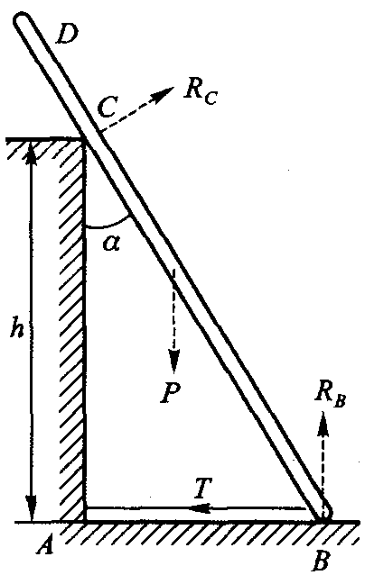
\includegraphics[width=0.25\linewidth]{figures/fig_6_25_1.png}\end{center}
\end{minipage}\par\vfill
\noindent\begin{minipage}{\textwidth}\ProblemHeading{习题}{6.26}
重为 $P$ 的杆 $AB$ 的端点 $A$、$B$ 分别靠在光滑的竖直面和水平面上，并由两根水平绳 $AD$ 和 $BC$ 拉住。绳 $BC$ 与杆 $AB$ 位于同一竖直平面内，杆的重力作用于其中点。令 $\alpha$ 为 $AB$ 与 $BC$ 的夹角，$\beta$ 为 $BC$ 与两支撑平面的交线所成的锐角（见图）。求两处支撑反力及两根绳的张力。
\begin{center}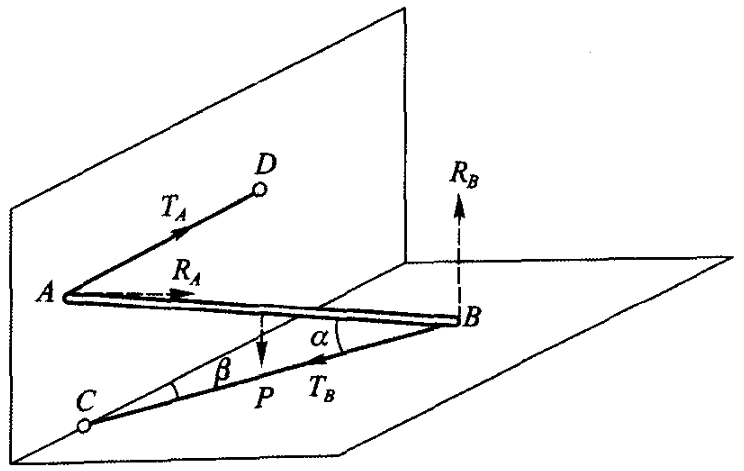
\includegraphics[width=0.38\linewidth]{figures/fig_6_26_1.png}\end{center}
\end{minipage}\par\vfill
\newpage
\noindent\begin{minipage}{\textwidth}\ProblemHeading{习题}{6.27}
长度均为 $l$ 的两根轻杆 $AC$、$BC$ 在上端 $C$ 铰接，下端 $A$、$B$ 支在光滑水平面上，并由绳 $AB$ 相连。在杆 $AC$ 的中点施加竖直向下的力 $F$。设两根杆与水平面所成的角均为 $\alpha$，求支撑反力、铰链反力和绳的张力。
\end{minipage}\par\vfill
\noindent\begin{minipage}{\textwidth}\ProblemHeading{习题}{6.28}
在北纬 $\lambda$ 处，一物体从距地面高度 $h$ 处相对于地面由静止释放。设当地重力加速度的大小为 $g$、地球自转角速度的大小为 $\Omega$，忽略空气阻力，只保留关于 $\Omega$ 的一阶项。求落地点相对于释放点竖直投影的水平偏移。
\end{minipage}\par\vfill
\newpage
\noindent\begin{minipage}{\textwidth}\ProblemHeading{习题}{6.29}
在北纬 $\lambda$ 处，一物体从地面以初速度 $\mathbf v_0$ 向上抛出。取 $x$ 轴沿当地子午线指北，$z$ 轴竖直向上；初速度位于 $xz$ 平面内，竖直分量为正。设当地重力加速度大小为 $g$、地球自转角速度大小为 $\Omega$，忽略空气阻力。求只保留 $\Omega$ 的一阶项时，物体落回地面处相对于忽略地球自转时的水平偏移。
\end{minipage}\par\vfill
\noindent\begin{minipage}{\textwidth}\ProblemHeading{习题}{6.30}
在纬度为 $\lambda$ 的地点研究一个可沿任意水平方向微振动的单摆（傅科摆）。设不考虑地球自转时的振动角频率为 $\omega_0$，地球自转角速度大小为 $\Omega$，且 $\Omega\ll\omega_0$。求地球自转对单摆微振动的影响，确定摆动轨迹在水平面内的转动速率及方向。
\end{minipage}\par\vfill
